\documentclass[10pt, letterpaper]{article}
\usepackage[cm]{fullpage}
\usepackage{algpseudocode}
\usepackage{algorithm}
\usepackage{graphicx}
\usepackage[section]{placeins}
\usepackage[table]{xcolor}
\usepackage{amsmath}
\usepackage[margin=0.7in]{geometry}
\usepackage{comment}
\usepackage{wrapfig}
\usepackage[demo]{graphicx}

\algrenewcommand\Return{\State \algorithmicreturn{} }%

\title{Tetanus - A Batch GCD RSA Cracker}
\author{Daiwei Chen \and Cole Houston}
\date{\today}

\begin{document}
\maketitle

\begin{abstract}
RSA is a widely used system for modern public key cryptography. It can be extremely secure, but there are several ways in which it can be implemented poorly. One such way is through weak generation of keys. This can happen when the seed used in the generation of the keys is not entirely random, which is the weakness that our program exploits. If several keys have the same seed, it is possible to deduce one of the prime numbers contained in the private key from the public key.  From there, it is possible to recreate the entire private key that should never be seen by the public in a strong implementation of RSA.
\end{abstract}

\section{RSA}
Let's quickly go over RSA, how it is possible to break it. RSA is usually cryptographically secure due to the complexity and difficulty to factor very, very large prime numbers. However, within the Public Component of RSA contains $N$, a result of the product between two (usually) large primes $p$ and $q$. However, if one could efficiently calcualte $p$ and $q$ from $N$, then it will be possible to reconstruct a RSA Private key. \\
\\
This means it is possible to perform Man In the Middle attacks against the cracked RSA Private Key target. Decrypt TLS encrypted traffic, or even authenticate SSH using the public key as well. Essentially, you become your target.

\section{Batch GCD}

\begin{wrapfigure}{r}{0.5\textwidth}
  \begin{center}
    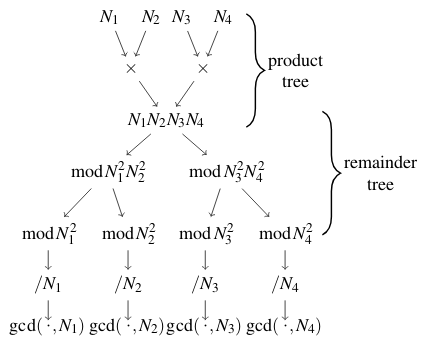
\includegraphics[width=0.48\textwidth]{batch-gcd-tree.png}
  \end{center}
  \caption{The Batch GCD Trees, being created and used.}
\end{wrapfigure}

Batch GCD is split into 3 main components: creation of the product tree, creation of the remainder tree, and finally, the GCD process.

\begin{enumerate}
\item Creation of the product tree. \\
  The base of the product tree is simply the RSA moduli. The product tree is created by multiplying 2 numbers to create a new layer, and keep multiplying every next 2 numbers together till you run out of numbers. On odd layers, simply add the final number to the end. Stop creating more layers until you reach the final number.
\item Creation of the remainder tree. \\
  The remainder tree is created by first using the final number of the product tree. Then, for each new layer, the $i/2$th product number in that layer is modded to with then $i$th number on the next layer of the product tree squared. This is a faster version of Batch-GCD, in the slower version, you simply create the final layer of the remainder tree by modding the final product tree number to each moduli.
\item Performing the GCD. \\
  Finally, for each moduli, find the GCD between each number on the final layer of the remainder tree divide by the modulus and the modulus itself.
\end{enumerate}

The complexity of Batch-GCD is $O(n(\lg{n})^2 \lg{\lg{n}})$ for the entire process.

\section{Reconstruction}
After vulnerable keys are identified by batch GCD, it is possible to reconstruct the RSA private key. $N$ is publicly available via the public key, and the batch GCD algorithm reveals either $p$ or $q$.  Since $N$ divided by $p$ will give you $q$, at this point all three numbers are available. The rest of the numbers needed for the private key are $e$, $d$, exponent 1, exponent 2, and coefficient.  $e$ can be found within the public key, so it is already available. $d$ can be calculated via an inverse modulus on (p-1)*(q-1). Exponent 1 can be found with d mod (p-1), and the second exponent is calculated the same way but with q rather than p. Lastly, the coefficient is found by (inverse of q) mod p. With those numbers, it is possible to reconstruct the entire RSA private key.

\section{Experimental Setup}
We have collected about 22,000 keys all together from 2 main sources for this project. First, we grabbed a datadump of about 10,000 moduli from a 2016 scan containing vulnerable moduli off the internet. Next, using a in-house tool tScanner, which performs TLS Handshakes with HTTPS servers to extract the certificate. Then, it extracts the public componet $N$ for Tetanus to attempt Batch-GCD cracking. The 12,000 keys were collected from about 2 entire days of scanning on one computer. The moduli are output by tScanner are all uniq, since duplicate moduli could raise a false positive for Tetanus.\\
\\
All moduli and gcd are saved and processed in hex. Within Rust, we used the Rug crate for arbitrary large number processing and math operations. The benchmark process is done on a single thread of an Intel i5-7200U (3.1 GHz), and 8 GB of ram with 8 GB of swap on SSD. 

\section{Results}
\begin{figure}[htp]
  \begin{center}
    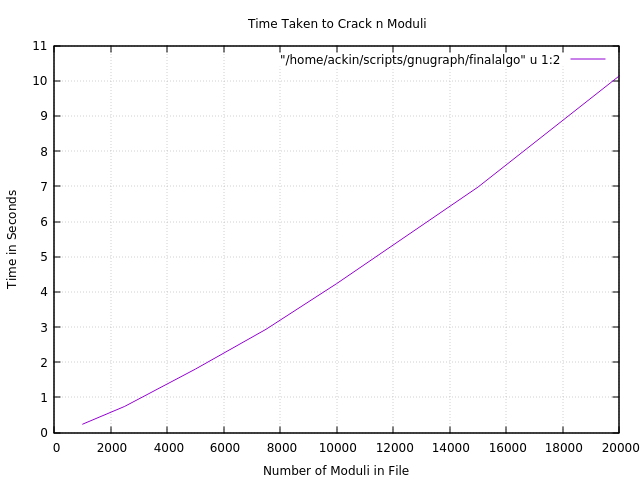
\includegraphics[scale=0.8]{batch-gcd-time.png}
    \caption{Results for n and t (in seconds)}
  \end{center}
\end{figure}

\section{Conclusions}
Batch-GCD works better with more keys, since there will be a higher chance of finding a GCD. However, network, memory, and storage is an issue; we simply just don't have enough time and resources to do a check of the entire IPv4 range. Once vulnerable keys are found, it is quick and easy to recreate the private key. Since it is not certain whether p or q is returned by Batch-GCD there are two possible private keys to reconstruct for each vulnerable key. Judging from the difference in the number of vulnerable keys found via the 2016 scan versus our 2019 scan there are fewer vulnerable keys in the world today. This is somewhat thanks to other exploits that have forced people to update their systems, but there are still several keys in the world that are vulnerable to the Batch-GCD attack.

\end{document}
